\chapter{Tracking library for the web (tracking.js)} % (fold)
\label{cha:tracking_library_for_the_web}

\section{Contextualization} % (fold)
\label{sec:tracking_library_for_the_web:Contextualization}

The desktop platform is the target environment most commonly addressed when developing AR systems. However, depending on the requirements of an AR application, the use of different execution platforms may be necessary. If the system has to be published to several users, the web platform shows to be more adequate, where the application is executed through the Internet in a web browser \cite{Pablo2013}.
The use of markerless tracking, which is based on natural features of the scene, is also gaining more space on web targeted AR applications for advertising. The medium used in this kind of application needs to be as appealing as possible in order to catch consumers' attention. Markerless tracking satisfies this requirement, since the idea of having a real scene augmented with virtual objects without any artificial elements such as markers added to the environment is very attractive. In addition, the product being advertised can be tracked and augmented with virtual elements.
Browsers are evolving very fast when compared to the the previous decade \cite{Hickson2013}. JavaScript language wasn't prepared to handle typed data structures \cite{TypedArray2013} able to manipulate raw binary data safely \cite{Canvas2013}, all the computational complexity required by AR algorithms was too much for that growing environment. Browsers weren't able to capture audio and video \cite{MediaCapture2013,WebRTC2013} natively, without plugin installation, an essential feature for AR applications. This reality has changed, this involves the use of several modern browser specifications as well as implementation of different computer vision algorithms and techniques into the browser environment taking advantage of all those modern APIs \cite{Hickson2013,WC2006}.

In this context, this dissertation aims to present the implementation and evaluation of a solution regarding tracking techniques for web targeted AR. The available algorithms and techniques can be used for different applications, such as, detecting faces, identifying objects and colors and tracking moving objects. The solution is called \textit{tracking.js}. Some optimizations are discussed and implemented in this work in order to achieve good results when compared with similar implementations in compiled languages.

\subsection{Related work} % (fold)
\label{sub:tracking_library_for_the_web:related_work}

There are not many web-based RA solutions available and registered in the literature. The ones available are mainly focused on fiducial markers \cite{Cho1998}, such as FLARToolKit \cite{Yan2011} and JSARToolkit \cite{JSARToolkit2011}, they both are ports of ARToolKit \cite{Hirokazu2002}. ARToolKit is a desktop library which is useful to make vision-based AR applications. The Metaio company developed Unifeye Viewer \cite{Metaio2009}, a proprietary plug-in for Flash \cite{Flash2013} that allows the utilization of markerless AR applications on the web. In order to run Flash based applications, the installation of its plugin is required. Third-party plugins, such as Flash, are in decadency on modern and mobile web browsers, instead JavaScript based solutions are preferred, since they can run in any modern browser without requiring any user effort of installing external software. Some smart-phones do not even support Flash plugin into their browsers, \eg\ Safari for mobile \cite{Safari2013} is one example of a mobile browser that has banned Flash.

\begin{enumerate}
    \item FLARToolKit: is a port of the well-known ARToolKit marker tracking library to ActionScript \cite{Flash2013}, which is the language utilized in the development of Flash applications for the web. This was the first initiative towards AR solutions for the web \cite{Pablo2013}. Using FLARToolKit, is possible to develop AR applications that run on a client's browser. A marker-based AR example for the web, developed for a marketing campaign of General Electric's company using FLARToolKit, is shown on Figure \ref{figure:flartoolkit}.

    \begin{figure}[!htb]
      \centering
      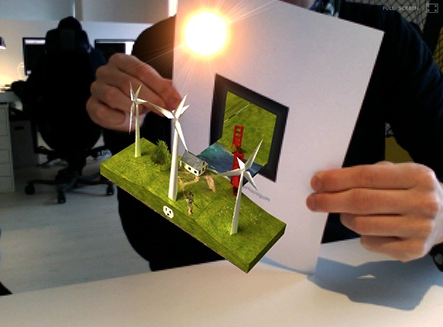
\includegraphics[width=240pt]{chapters/tracking_library_for_the_web/flartoolkit.png}
      \caption{Marker based AR for the web using FLARToolKit.}
      \label{figure:flartoolkit}
    \end{figure}

    \item JSARToolkit: is a JavaScript port of FLARToolKit, operating on canvas images and video element contents, provides another marker tracking library. This was the first, open-source, JavaScript-based, AR solution available for the web. A marker-based AR example for the web using JSARToolKit is shown on Figure \ref{figure:jsartoolkit}.

    \begin{figure}[!htb]
      \centering
      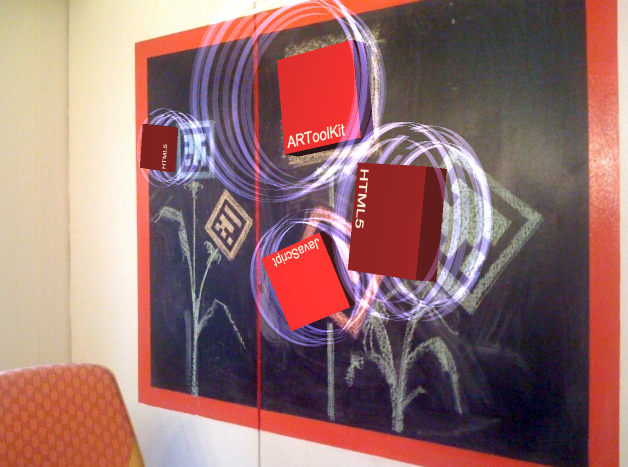
\includegraphics[width=240pt]{chapters/tracking_library_for_the_web/jsartoolkit.png}
      \caption{Marker-based AR for the web using JSARToolKit.}
      \label{figure:jsartoolkit}
    \end{figure}

    \item Unifeye Viewer: from Metaio company, it offers a robust markerless tracking solution for the web. Unifeye \cite{Metaio2009} also depends on Flash plugin in order to run on web browsers. A similar example of General Electric's marker-based solution, this time markerless based, is shown on Figure \ref{figure:unifeyeviewer}. Note that the 3D image is projected over a magazine cover instead of a fiducial marker.

    \begin{figure}[!htb]
      \centering
      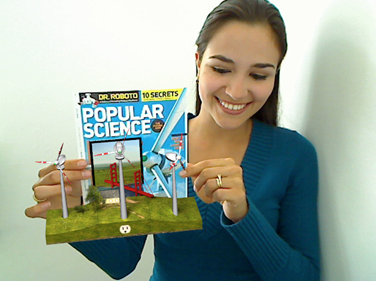
\includegraphics[width=240pt]{chapters/tracking_library_for_the_web/unifeyeviewer.png}
      \caption{Markerless example of image projected over a magazine cover using Unifeye Viewer solution.}
      \label{figure:unifeyeviewer}
    \end{figure}
\end{enumerate}

There is a disadvantage of using marker-based AR. Depending on an artificial marker in order to augment the scene with virtual elements is counterintuitive. Commonly, web applications are utilized by novice users that do not have sufficient technical knowledge to perform manual setup, such as printing fiducial markers or performing manual initialization for the tracking. FLARToolKit and JSARToolkit are both marker-based techniques, using Flash and JavaScript, respectively. FLARToolKit has one more issue which is dependency on Flash plugin installation. Unifeye Viewer by Metaio was the only existing solution that provided markerless tracking for the web, although it uses Flash, excluding it from a potential competitor of \textit{tracking.js}. Markerless tracking techniques aim at not depending on any artificial marker or advanced user initialization. The space on web-targeted AR applications for advertising is on the rise and the medium used in this kind of application needs to be as appealing as possible \cite{Pablo2013} making markerless tracking a suitable technique to such applications.

The solution proposed in this dissertation, \textit{tracking.js}, provides the first known, open-source, markerless tracking solution for the web that runs entirely in JavaScript and HTML5.

% subsection related_work (end)

\subsection{Library modules} % (fold)
\label{sub:tracking_library_for_the_web:library_modules}

The proposed library is divided in modules in order to allow extension and addition of new features, such as new RA techniques or math utilities. For a better understanding of the library architecture, the current implementation is divided in two packages separating base from visual tracking classes. Base classes modules are shown in Figure \ref{figure:base_classes} and visual tracking classes in Figure \ref{figure:visual_tracking_classes}.

To develop AR applications using only raw JavaScript APIs \cite{MDN2013} could be too verbose and complex, \eg\ capturing users' camera and reading its array of pixels. The big amount of steps required for a simple task makes web developers life hard when the goal is to achieve complex implementations. Some level of encapsulation is needed in order to simplify development. The proposed library provides encapsulation for common tasks on the web platform.

The two main available packages splits base from visual tracking classes. Furthermore, each class of those packages are described. Let's start with the base classes:

\begin{enumerate}
  \item Math: provides common math utilities optimized for the web, such as geometry, linear algebra \cite{Hartley2004} and hamming operations. Typed arrays are used in order to optimize performance, see subsection \ref{sub:basic_concepts:web:javascript_typed_arrays} for more information about typed arrays.
  \item Attribute: allows developers to add attributes to any class through an Attribute interface. The interface adds get and set methods to your class to retrieve and store attribute values, as well as support for change events that can be used to listen for changes in attribute values.
  \item DOMElement: provides a way to create, and manipulate HTML DOM nodes \cite{WC2006}. Each DOMElement instance represents an underlying DOM node. In addition to wrapping the basic DOM API and handling cross browser issues, Nodes provide convenient methods for managing styles and subscribing to events.
  \item Canvas: provides an utility class to create, and manipulate HTML5 canvas element. Each Canvas instance represents an underlying canvas DOM node. In addition to wrapping the basic DOM API, also provides methods to extract via \textit{getImageData} method, to loop via \textit{forEach} method, and to set the canvas array of pixels via \textit{setImageData} method.
  \item Video: provides an utility class to create, and manipulate HTML5 video element. Each Video instance represents an underlying video DOM node. In addition to wrapping the basic DOM API, also provides methods to \textit{play}, \textit{pause} and register tracker algorithms via \textit{track} method. See subsection \ref{sub:basic_concepts:web:audio_and_video} for more information about video element.
  \item VideoCamera: extends all functionalities from Video class with the addition of capturing the user camera via \textit{capture} method. The underlying implementation uses WebRTC \cite{WebRTC2013} and Media Capture and Streams \cite{MediaCapture2013} specifications.
\end{enumerate}

Visual tracking classes include several computer vision algorithms, such as FAST \cite{RostenFaster2010}, BRIEF \cite{Calonder2010} implementations, homography estimation and others. As the library grows, many other computer vision algorithms are added to the library, such as 3D pose calculation.

\begin{enumerate}
  \item FAST: provides an implementation of Features from Accelerated Segment Test (FAST) \cite{Rosten2010} for features detection via \textit{findCorners(data, threshold)} method, where $data$ is the \textit{ImageData} of the canvas frame. It also depends on a $threshold$ argument. The pixel at $p$ is the center of a candidate corner classified if the concentric contiguous arcs around $p$ are different by more than the $threshold$, see Figure \ref{figure:fast}.

  \item BRIEF: provides an implementation of Binary Robust Independent Elementary Features (BRIEF) \cite{Calonder2010} for feature extraction via \textit{getDescriptors(data, corners)} method and matching via \textit{match(c1, d1, c2, d2)}, where $data$ is an \textit{ImageData}, and $c1$ and $c2$ are the \textit{found corners} array return by \textit{FAST.findCorners} method and $d1$ and $d2$ are feature descriptors array return by \textit{BRIEF.getDescriptors} method.
  \item RANSAC: provides an interface used to achieve robust estimation method for homographies and camera pose. A Homography estimation is available that inherits from RANSAC \cite{Hartley2004} base funcionality.
  \item Homography: provides an API to estimate a homography matrix $H$ between images by finding feature correspondences in those images.
  \item ViolaJones: provides scanning detector algorithms for robust and extremely rapid object detection.
  \item Color: provides a fast and robust solution for color blob detection.
\end{enumerate}

\begin{figure}[!htb]
    % \tikzumlset{font=\scriptsize}
    \begin{tikzpicture}
        \begin{umlpackage}{Base classes}

            \umlclass[y=-50pt,x=190pt]{Math}{}{
              createIdentityMatrix(size) : Matrix\\
              distance(x1, y1, x2, y2) : Number\\
              getDeterminant(Matrix) : Number\\
              getInverse(Matrix) : Matrix\\
              hammingDistance(n1, n2) : Number\\
              hammingWeight(number) : Number\\
              ...
            }

            \umlclass{Attribute}{}{
              get(name) : Object\\
              set(name, value) : void \\
            }

            \umlclass[y=-100pt]{DOMElement}{
              width : Number\\
              height : Number\\
              visible : boolean\\
            }{
              show() : void\\
              hide() : void \\
            }

            \umlclass[y=-220pt,x=180pt]{Canvas}{
              context : Object
            }{
              forEach(data, callback) : void\\
              getImageData(x, y, width, height) : ImageData \\
              setImageData(data, x, y) : void\\
            }

            \umlclass[y=-335pt]{Video}{}{
              play() : void\\
              pause() : void\\
              track(tracker) : void \\
              getVideoCanvasImageData(x, y, width, height) : ImageData \\
            }

            \umlclass[y=-335pt,x=220pt]{VideoCamera}{}{
              capture() : void \\
            }

        \end{umlpackage}

        \umlinherit[geometry=-|]{DOMElement}{Attribute}
        \umlinherit[geometry=-|]{Canvas}{DOMElement}
        \umlinherit[geometry=-|]{Video}{DOMElement}
        \umlinherit[geometry=|-]{VideoCamera}{Video}
    \end{tikzpicture}
    \caption{Base classes of tracking.js library.}
    \label{figure:base_classes}
\end{figure}

\begin{figure}[!htb]
    % \tikzumlset{font=\scriptsize}
    \begin{tikzpicture}
        \begin{umlpackage}{Visual tracking classes}

            \umlclass{FAST}{}{
              findCorners(data, threshold) : Array\\
            }

            \umlclass[y=-70pt]{BRIEF}{}{
              getDescriptors(data, corners) : Array\\
              match(c1, d1, c2, d2) : Array\\
            }

            \umlclass[y=-150pt]{ViolaJones}{}{
              find() : Array\\
              evalStage() : boolean\\
            }

            \umlclass[y=-225pt]{Color}{}{
              find() : Array\\
            }

            \umlclass[x=200pt]{RANSAC}{}{
              find(matches) : void\\
              score() : Number\\
            }

            \umlclass[y=-90pt,x=200pt]{Homography}{}{
                score(H, matches) : Number\\
            }

        \end{umlpackage}

        \umlinherit[geometry=-|]{Homography}{RANSAC}
    \end{tikzpicture}
    \caption{Visual tracking classes of tracking.js library.}
    \label{figure:visual_tracking_classes}
\end{figure}

\clearpage

% subsection library_modules (end)

% section contextualization (end)

\section{Markerless tracking algorithm} % (fold)
\label{sec:tracking_library_for_the_web:marker_less_tracking_algorithm}

\subsection{Contextualization} % (fold)
\label{sub:tracking_library_for_the_web:marker_less_tracking_algorithm:contextualization}

The basic difference between markerless and marker-based tracking is that the first does not require artificial markers put on the environment in order to estimate camera pose. Markerless tracking can, in theory, use any part of the scene as a reference to position virtual objects, although in practice, some restrictions may apply, depending on the specific technique used. Several algorithms for markerless tracking are available in the literature \cite{Teichrieb2007}. Some of them require a previous knowledge about the environment, such as a digital model of a real object to be tracked, the texture of a region of the scene, etc. These methods are known as model based. Other techniques can make an online estimate of the topology of the environment, using only different frames captured from the scene by a moving camera for registration of the virtual objects. These techniques are called Structure from Motion (SfM) and are often more complex and require more processing power to achieve real-time frame rates. Since this work aims to develop some web targeted markerless AR solutions, the keypoint-based technique was chosen for tracking purposes, which is a model based technique described in \cite{Teichrieb2010}. It is a tracking-by-detection technique, being able to detect the target object at every frame without any previous estimate of its pose, allowing automatic initialization and recovery from failures.

% subsection contextualization (end)

\subsection{Feature detector} % (fold)
\label{sub:tracking_library_for_the_web:marker_less_tracking_algorithm:feature_detector}

This technique relies on detecting individual features across images and are therefore easy to increase robustness against partial occlusions or matching errors. Illumination invariance is also simple to achieve. Feature points detection is used as the first step of many vision tasks such as tracking, localization, image matching and recognition \cite{Lepetit2005}. In this work we call ``feature'' or ``keypoint'' to refer to a point of interest in two dimensions (Figure \ref{figure:keypoints}).

\begin{figure}[!htb]
  \centering
  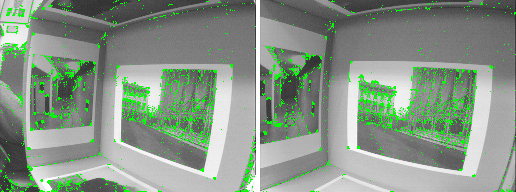
\includegraphics[width=380pt]{chapters/tracking_library_for_the_web/keypoints.png}
  \caption{Image features detected on two different frames, green pixels represent found keypoints.}
  \label{figure:keypoints}
\end{figure}

For each frame, the object features are matched by localizing feature templates in search windows around hypothesized locations \cite{Lepetit2005}. The method to extract feature points proposed is Features from Accelerated Segment Test (FAST) \cite{Rosten2010,RostenFaster2010}. FAST hypothesizes the matches using corner detection. A large number of corner detectors exists in the literature. However, in order to allow AR solutions to be developed on top of this work, we have a strong interest in real-time-frame-rate applications which computational resources are required requisites. The approach proposed by FAST allows the detector to produce a suite of high-speed detectors which we currently use for real-time tracking and AR label placement \cite{Calonder2010}. In particular, it is still true that when processing live video streams at full frame rate, existing feature detectors leave little if any time for further processing, despite the consequences of Moore's Law \cite{Rosten2010}.

A number of detectors described below computes a corner response: (1) Edge-based corner detectors, correspond to the boundary between two regions; (2) Gray-level-derivative-based detectors, the assumption that corners exist along edges is an inadequate model for patches of texture and point-like features, and is difficult to use at junctions. Therefore a large number of detectors operate directly on gray level images without requiring edge detection; and (3) Direct-gray-level detectors, another major class of corner detectors works by examining a small patch of an image to see if it ``looks'' like a corner \cite{Rosten2010}.

The dissertation choice was (3) Direct-gray-level detectors, since its robustness against partial occlusions or matching errors and illumination invariance is simple to achieve and the computational complexity of the technique is low.
Despite the design of FAST for speed, this detector has excellent repeatability, in addition, a variation of FAST technique that uses machine learning (FAST-ER \cite{RostenFaster2010}) can be implemented in a future work, providing dramatic improvements in repeatability over FAST-$9$ (especially in noisy images). It works by testing a small patch of an image to see if it could be a corner. The detector is evaluated using a circle surrounding the candidate pixel, the test is based on whether the concentric contiguous arcs around the pixel are significantly different from the central pixel $p$. To classify $p$ as a corner should exist a set of $n$ contiguous pixels in the circle which are all brighter than the intensity of the candidate pixel $I_{p} + t$ (threshold), or all darker than $I_{p} - t$. The number of contiguous tested pixels could vary accordingly, being more common to be FAST-$12$ or FAST-$9$. Empirically, FAST-$9$ showed to have a good repeatability and a better efficiency on the web. The repeatability of found feature points is also important because it determines whether the technique is useful in a real-world application.

This detector itself exhibits high performance, but there are several weaknesses: (1) This high-speed test does not reject as many candidates; (2) The efficiency of the detector will depend on the ordering of the questions and the distribution of corner appearances; and (3) Multiple features are detected adjacent to one another \cite{Rosten2010}.

On Figure \ref{figure:fast}, the highlighted squares are the pixels used in the corner detection. The pixel at $p$ is the central pixel. The arc is indicating that the dashed line passes through FAST-$n$, let $n$ be $9$ or $12$ contiguous pixels which are brighter or darker than $p$ \cite{Rosten2010}.

\begin{figure}[!htb]
  \centering
  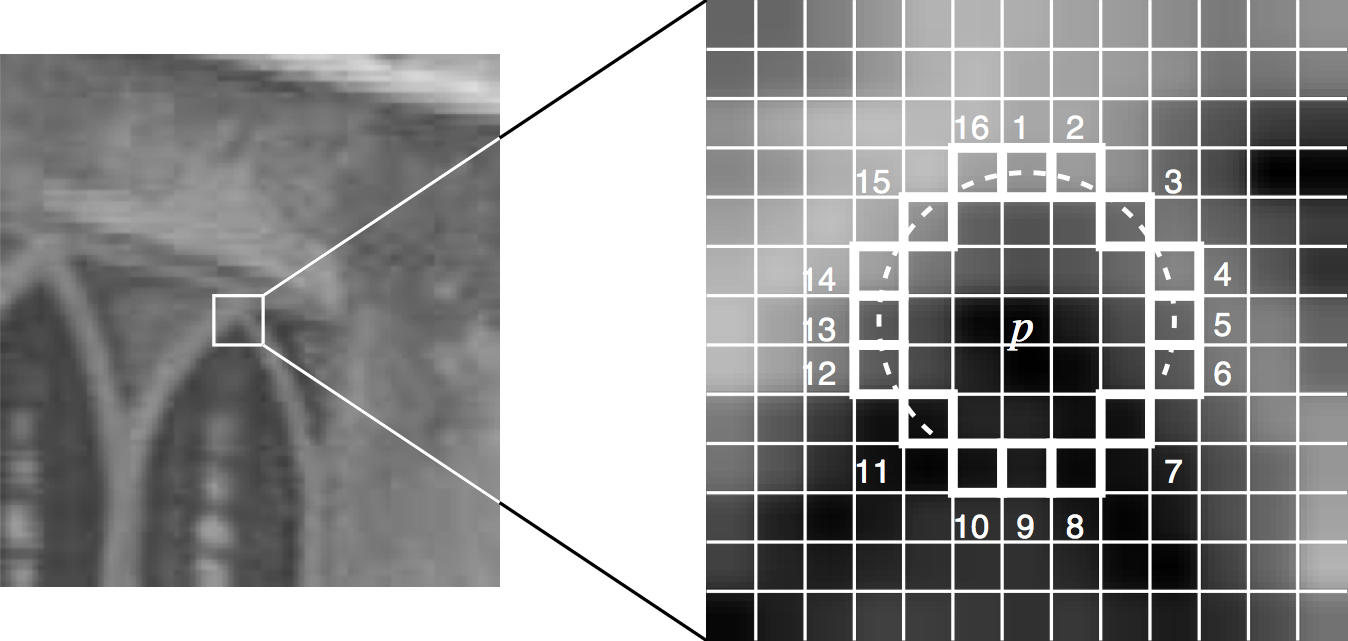
\includegraphics[width=380pt]{chapters/tracking_library_for_the_web/fast.png}
  \caption{Point segment test corner detection in an image patch \cite{Glass2013}.}
  \label{figure:fast}
\end{figure}

% subsection feature_detector (end)

\subsection{Feature extractor} % (fold)
\label{sub:tracking_library_for_the_web:marker_less_tracking_algorithm:feature_extractor}

To estimate motion, one can then match sets of features \{$m_{i}$\} and \{$m'_{j}$\} extracted from two images taken from similar, and often successive, viewpoints. A classical procedure \cite{Calonder2010} runs as follows. For each point \{$m_{i}$\} in the first image, search in a region of the second image around location \{$m_{i}$\} for point \{$m'_{j}$\}. The search is based on the similarity of the local image windows, also knowns as kernel windows, centered on the points, which strongly characterizes the points when the images are sufficiently close \cite{Lepetit2005}.

\begin{figure}[!htb]
  \centering
  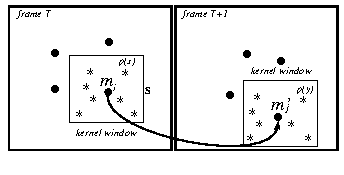
\includegraphics[width=\linewidth]{chapters/tracking_library_for_the_web/BRIEF.pdf}
  \caption{BRIEF \cite{Lepetit2005} feature extractor.}
  \label{figure:BRIEF}
\end{figure}

The feature matching used in the case studies performed in this work searches for correspondent points in the current frame. Only points that are highly descriptive invariant features, called keypoints, are tested. After the keypoints are detected they need to be described and the respective matching point should be found. Since web and handled devices have limited computational power, having local descriptors that are fast to compute, to match and being memory efficient are important aspects, and for that reason, it was used an efficient method called Binary Robust Independent Elementary Features (BRIEF).

To generate the binary string for each keypoint found in the smoothed frame, the individual bits are obtained by comparing the intensities of pairs of points, $(\textbf{p}; x, y)$, represented by $\ast$ symbol on Figure \ref{figure:BRIEF}, along the kernel window centered on each keypoint without requiring a training phase.
Empirically, this technique shows that $256$ or even $128$ bits \cite{Calonder2010}, often suffice to obtain very good matching results. In order to have better recognition rates, the best spatial arrangement of the tested (\textbf{x}, \textbf{y})-pairs of points are reached when selected based on an isotropic Gaussian distribution. Computing the Gaussian distribution can be time consuming. As an optimization proposed by this work, the Gaussian distribution could be simply replaced by a uniform version of JavaScript \textit{Math.random()} function. Function \textit{Math.random()} should return an evenly-distributed variable $X$ such that $0.0 \le X < 1.0$ and $X$ is commonly seeded from the current time \cite{International2009}. The locations of (\textbf{x}, \textbf{y})-pairs are evenly distributed over the patch and tests can lie close to the patch border, \ie\ $(-\frac{S}{2},\frac{S}{2})$.

To generate the binary strings it is defined the test $\tau$ on patch \textbf{p} of size \textbf{S $\times$ S} as

$$\tau(\textbf{p}; x, y) :=
\begin{cases}
  1 &\mbox{if}\quad \textbf{p(x)} < \textbf{p(y)},\\
  0 &\mbox{otherwise}
\end{cases}$$

where \textbf{p(x)} is the pixel intensity. The set of binary tests is defined by the $n_{d}$ (\textbf{x}, \textbf{y})-location pairs uniquely chosen during the initialization. The $n_{d}$-dimensional bit-string is our BRIEF descriptor for each keypoint

$$f_{n_{d}}(\textbf{p}) := \sum_{1 \le i \le n_{d}} 2^{i-1} \tau(\textbf{p}; x, y).$$

In \cite{Calonder2010}, $n_{d}= 128, 256, 512$ were used in the tests and any of those values yield good compromises between speed, storage efficiency, and recognition rate. In this work, $n_{d}= 128$ was used, since it presented good matching results and performance. The number of bytes required to store the descriptor can be calculated by $k = n_{d}/8$, proving that BRIEF is also a memory-efficient method. Detailed results can be found in Chapter \ref{cha:evaluation}.

Once each keypoint is described with its binary string, they need to be compared with the closest matching point. Distance metric is critical to the performance of intrusion detection systems. Thus using binary strings reduces the size of the descriptor and provides an interesting data structure that is fast to operate whose similarity can be measured by the Hamming distance which, on desktop implementations, the computation time could be driven almost to zero by using the POPCNT instruction from SSE4.2 \cite{Intel2007}. Only the latest Intel Core i7 CPUs support this instruction.

The Hamming distance is an important step on feature matching, it provides a fast and memory-efficient way to calculate distance between binary strings. Given two image patches $x$ and $y$, denote their binary descriptors as $b(x) \in \{0,1\}^n$ and $b(y) \in \{0,1\}^n$ respectively. Then their Hamming distance is computed by:
$$Ham(x, y)=\sum_{i=1}^{n}b_i(x)\otimes b_i(y)$$
in which $n$ is the dimension of binary descriptor and $\otimes$ stands for bitwise exclusive OR operation. According to the definition of Hamming distance, all the elements of a binary descriptor contribute equally to the distance. From the hamming distance, the Hamming weight can be calculated. It is used to find the best feature point match. Here, is generalized the Hamming distance to the weighted Hamming:
$$WHam(x, y)=\sum_{i=1}^{n}w_i(b_i(x)\otimes b_i(y))$$
where $w_i$ is the weight of the $i$th element. The goal is to learn $w_i,i=1,2\cdots,n$ for the binary descriptor (BRIEF) based on a set of feature points. By assigning different weights to binary codes, what we expect is to obtain a distance space in which the distances of matching patches are less than those of non-matching patches.

% subsection feature_extractor (end)

\subsection{Homography estimation} % (fold)
\label{sub:tracking_library_for_the_web:marker_less_tracking_algorithm:homography_estimation}

Typically, homographies are estimated between images by finding feature correspondences on them. A 2D point $(x,y)$ in an image can be represented as a 3D vector $\textbf{x} = (x_1, x_2, x_3)$ where $x = \frac{x_1}{x_3}$ and $y = \frac{x_2}{x_3}$ \cite{Homography2009}. This is called the homogeneous representation of a point and it lies on the projective plane $P^2$. A homography is an invertible mapping of points and lines on the projective plane $P^2$. Hartley and Zisserman \cite{Hartley2004} provide the specific definition that a homography is a mapping from $P^2$ → $P^2$ which is a projectivity if and only if there exists a non-singular $3\times3$ matrix $H$ such that for any point in $P^2$ represented by vector $\textbf{x}$ it is true that its mapped point equals $H\textbf{x}$. It should be noted that $H$ can be changed by multiplying by an arbitrary non-zero constant without altering the projective transformation. Thus $H$ is considered a homogeneous matrix and only has $8$ degrees of freedom even though it contains $9$ elements.

The method chosen to solve the homography estimation was the Direct Linear Transformation (DLT) \cite{Impa2009,Hartley2004} algorithm. The DLT algorithm is a simple algorithm used to solve for the homography matrix $H$ given a sufficient set of point correspondences \cite{Homography2009}.

Since we are working in homogeneous coordinates, the relationship between two corresponding points $\textbf{x}$ and $\textbf{x'}$ can be re-written as \cite{Homography2009}:
$$c\begin{pmatrix}u\\ v\\ 1\\\end{pmatrix} = H\begin{pmatrix}x\\ y\\ 1\\\end{pmatrix}, \;\; H=\begin{pmatrix}h1 & h2 & h3\\ h4 & h5 & h6\\ h7 & h8 & h9\\\end{pmatrix},$$
where $c$ is any non-zero constant, $(\; u \; v \; 1 \;)^T$ represents $\textbf{x'}$, $(\; x \; y \; 1 \;)^T$ represents $\textbf{x}$. Dividing the first row of the above equation by the third row and the second row by the third row we get the following two equations:

\begin{equation}
\label{eq:homography1}
-h1x-h2y-h3 +(h7x+h8y+h9)u=0
\end{equation}
\begin{equation}
\label{eq:homography2}
-h4x-h5y-h6 +(h7x+h8y+h9)v=0
\end{equation}

Equations (\ref{eq:homography1}) and (\ref{eq:homography2}) can be written in matrix form as $A_i\textbf{h}=0$. Where,

$$A_i=\begin{pmatrix}-x & -y & -1 & 0 & 0 & 0 & ux & uy & u\\0 & 0 & 0 & -x & -y & -1 & vx & vy & v\end{pmatrix}$$

and

$$\textbf{h}=\begin{pmatrix}h1 & h2 & h3 & h4 & h5 & h6 & h7 & h8 & h9\end{pmatrix}.$$

Since each point correspondence provides $2$ equations, $4$ correspondences are sufficient to solve for the $8$ degrees of freedom of $H$. JavaScript-typed arrays, defined in Section \ref{sub:basic_concepts:web:javascript_typed_arrays}, were used in the homography estimation implementation for better performance results.

% subsection homography_estimation (end)

\subsection{Random sample consensus (RANSAC)} % (fold)
\label{sub:tracking_library_for_the_web:marker_less_tracking_algorithm:ransac}

RANSAC (Random Sample Consensus) \cite{Hartley2004} is an iterative method to estimate parameters of a mathematical model from a set of observed data which contains outliers. It is a non-deterministic algorithm in the sense that it produces a reasonable result only with a certain probability, with this probability increasing as more iterations are allowed. It is the most commonly used robust estimation method for homographies according to \cite{Homography2009}. The idea of the algorithm is pretty simple; for a number of iterations, a random sample of $4$ correspondences is selected and a homography $H$ is computed from those four correspondences. Each other correspondence is then classified as an inlier or outlier depending on its concurrence with $H$. After all of the iterations are done, the iteration that contained the largest number of inliers is selected. The matrix $H$ can then be recomputed from all of the correspondences that were considered as inliers in that iteration \cite{Homography2009}.

One important step when applying the RANSAC algorithm described above is to decide how to classify correspondences as inliers or outliers. In the implementation for the web only assigning the geometric distance threshold, $t$, between $\textbf{x'}$ and $H\textbf{x}$ was enough. Hartley and Zisserman \cite{Hartley2004} provide more details about RANSAC.

Another issue is to decide how many iterations to run the algorithm, it is not required to try every combination of 4 correspondences. The goal becomes to determine the number of iterations, $N$, that ensures with a probability $p$ that at least one of the random samples will be free from outliers. $N=100$ was used on the web implementation.

% subsection ransac (end)

% section marker_less_tracking_algorithm (end)

\section{Rapid object detection (Viola Jones)} % (fold)
\label{sec:tracking_library_for_the_web:rapid_object_detection}

\subsection{Contextualization} % (fold)
\label{sub:tracking_library_for_the_web:rapid_object_detection:contextualization}

Rapid Object Detection technique, much known as Viola Jones \cite{Viola2001}, brings together new algorithms and insights to construct a library for robust and extremely rapid object detection. What has motivated this technique to be added to \textit{tracking.js} library was the task of face detection. The algorithm implementation became robust enough to detect any training data, not only for faces. Currently, \textit{tracking.js} supports, face, eyes, upper body and palm detection.

In order to scan faces, eyes or palm from images, a training phase is required. The training phase generates cascading stages. The cascade is constructed by training classifiers using AdaBoost \cite{Viola2001} and then adjusting the threshold to minimize false negatives. OpenCV library \cite{Bradski2000} has some open-source training data, therefore doubling efforts on training is unnecessary, \ie\ the face training set consisted of 4916 faces, extracted from images downloaded during a random crawl of the world wide web \cite{Viola2001}. Those faces were scaled and aligned to a base resolution of $24$ by $24$ pixels, see Figure \ref{figure:viola_training}. Training is not the focus of this work, the algorithm to scan the faces is. The training data itself is useless if a Scanning Detector is not available, the scanning is what makes the rapid object detection.

\begin{figure}[!htb]
  \centering
  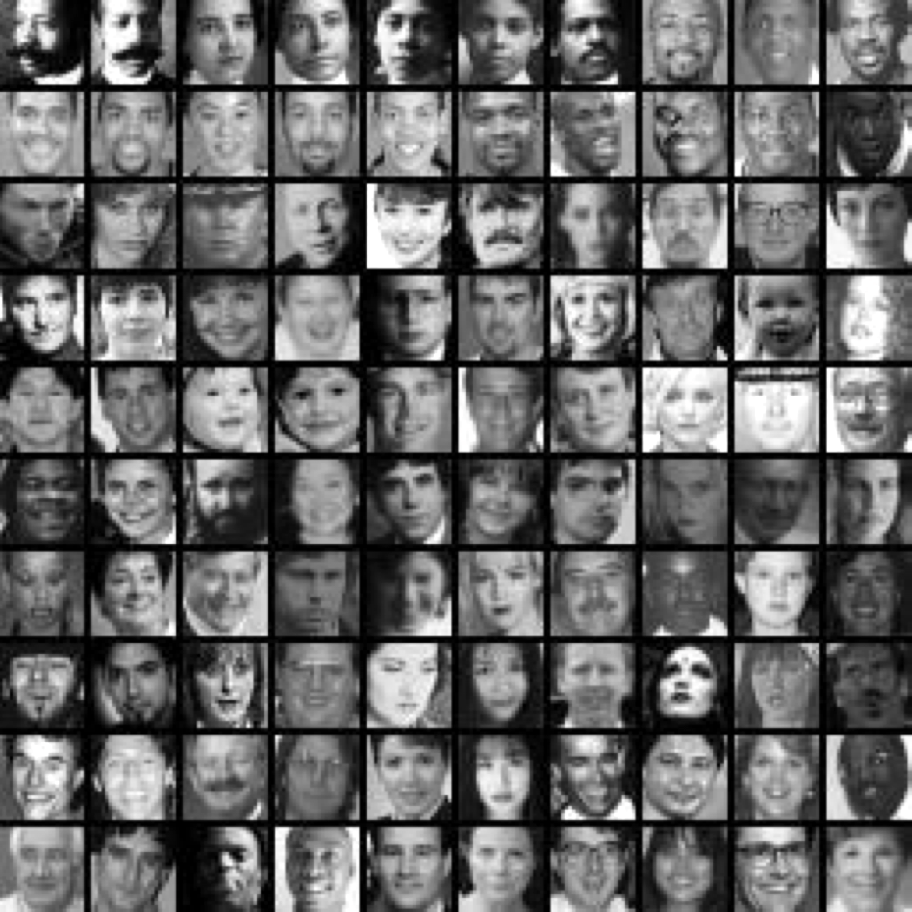
\includegraphics[width=240pt]{chapters/tracking_library_for_the_web/viola_training.png}
  \caption{Example of frontal upright face images used for training.}
  \label{figure:viola_training}
\end{figure}

A scanning detector was implemented in JavaScript and is available on \textit{tracking.js}. The training data used is from OpenCV library converted from Extensible Markup Language (XML) \cite{Bray2013} to JavaScript Object Notation (JSON) \cite{Crockford2013}. JSON has much superior performance since it is interpreted by JavaScript language. The results of the JavaScript implementation can be used in real-time applications, the detector runs at 15 frames per second. For more information about performance see Chapter \ref{cha:evaluation}.

The overall idea of the detection process is that it uses a degenerate decision tree, what Viola and Jones \cite{Viola2001} call ``cascade''. A positive result from the first classifier triggers the evaluation of a second classifier which has also been adjusted to achieve very high detection rates. A positive result from the second classifier triggers a third classifier, and so on. The main steps of the scanning algorithm are:

\begin{enumerate}
  \item Create or scale a squared block, initially set to $20\times20$ pixels, by $1.25$ per iteration;
  \item Loop the squared block by $\Delta$ pixels over the image;
  \item For each squared block location, loop the decision tree and evaluate each stage;
  \item A positive result of the stage triggers the next stage, otherwise stops the stages loop;
  \item If all stages were positively evaluated store that rectangle as a possible face;
  \item Once the decision tree is done, group the overlapping rectangles;
  \item Find the best rectangle of each the group to represent the face. This phase is also known as ``merging phase''.
\end{enumerate}

The final detector is scanned across the image at multiple scales and locations of the image. This process makes sense because the features can be evaluated at any scale with the same cost \cite{Viola2001}. Good results were obtained using a scale factor of $1.25$. Subsequent locations are obtained by shifting the window some number of pixels $\Delta$, for a better accuracy $\Delta=1$ is recommended. We can achieve a significant speedup by setting $\Delta=2$ with only a slight decrease in accuracy, thus this value was set as default value of the JavaScript implementation.

Viola and Jones \cite{Viola2001} proposed the found rectangles be partitioned into a disjoint set data structure. Two detections are in the same subset if their bounding regions overlap. The corners of the final bounding region are the average of the corners of all detections in the set. In order to perform well on the web, some optimizations were made in the implementation level of the scanning detector. The disjoint set was replaced by an alternative logic that is called ``Minimum Neighbor Area Grouping'' by this dissertation. Minimum Neighbor Area Grouping has $O(N^2)$ performance \cite{black2007big} and consists in a loop trough the possible rectangle faces returned by the scanning detector. For each step of the loop compare the current rectangle with all other not yet compared rectangles. If the rectangle area overlaps more than $\eta$ with the compared ones, by default $\eta=0.5$ (or $50\%$), select the smallest rectangle in area of the comparison. Using the smallest rectangle guarantees that the best match is much centralized in the face.

For more information about the JavaScript implementation, such as evaluation and results, see Chapter \ref{cha:evaluation}.

% subsection contextualization (end)

% section rapid_object_detection (end)

\section{Color tracking algorithm} % (fold)
\label{sec:tracking_library_for_the_web:color_tracking_algorithm}

\subsection{Contextualization} % (fold)
\label{sub:tracking_library_for_the_web:color_tracking_algorithm:contextualization}

Colors are everywhere in every single object. Being able to handle colored objects to control your browser through the camera is very appealing. For that reason, \textit{tracking.js} implemented a basic color tracking algorithm that resulted in an real-time frame rate trough a simple and intuitive API.
Color has been widely used in real-time tracking systems \cite{Paschos2001}. It offers several significant advantages over geometric cues such as computational simplicity, robustness under partial occlusion and illumination, rotation, scale and resolution changes.

In the tracking system implemented, the color blobs are being tracked. The notion of blobs as a representation for image features has a long history in computer vision and has had many different mathematical definitions. It may be a compact set of pixels that share a visual property that is not shared by the surrounding pixels \cite{Kravtchenko1999}. This property could be color, texture, brightness, motion, shading, a combination of these, or any other salient spatio-temporal property derived from the signal, in our case the image sequence.
Colour perception is a difficult and little understood problem, which seems to defy even the most ingenious mathematical expressions. Evaluating color differences is subjective: when asked to pick the ``closest'' match for a specific color from a small palette, the selections by test persons turned out to be different, therefore automating a color tracking technique is not as trivial as finding the specific RGB \cite{Gonzalez2007} value to be classified as a pixel of interest.

% subsection contextualization (end)

\subsection{Color difference evaluation} % (fold)
\label{sub:tracking_library_for_the_web:color_tracking_algorithm:color_difference_evaluation}

When a true color (photographic) image is mapped to a reduced palette, every true-color pixel must be mapped to the palette entry that comes closest to original color.
There are different ways to evaluate color difference, \ie\ large color difference (LCD), small color difference (SCD), and threshold color difference (TCD), they can use ratio judgment, pair comparison, and threshold \cite{Li2003}. In the latter, the difference between the original color and the quantized color should remain below some threshold. The quantization method implemented in this work determines whether the color is close to the tracked color by a threshold based on Euclidean distance.

Mapping a RGB color in an orthogonal three-dimensional space, the distance between two colors is denoted by the Euclidean distance $\|C_1-C_2\|$. For a three-dimensional space (with dimensions R, G and B) the Euclidean distance between two points is calculated as follows:

$$\|C_1-C_2\|=\sqrt{(C_{1,R}-C_{2,R})^2 + (C_{1,G}-C_{2,G})^2 + (C_{1,B}-C_{2,B})^2}.$$

Graphic applications for computers usually employ the Red-Green-Blue (RGB) color space. This model maps well to the way the common Cathode Ray Tube (CRT) and Liquid-Crystal Display (LCD) display works. These displays have three kinds of elements that emit red, green or blue light. Another advantage of the RGB model is that it is a three-dimensional orthogonal space, precisely what we need for the Euclidean distance function.

To determine if the pixel represents a possible color it should be inside the tracked color neighborhood and $\|C_1-C_2\|$ must be lower than a configurable $threshold=100$. Imagine that the tracked color $C_1$ is the center of a sphere in a three-dimensional space, any point $C_2$ around $C_1$ that its Euclidean distance is lower than a $threshold$ is considered a color that ``looks like'' $C_1$. Figure \ref{figure:rgb_space} exemplifies a color neighborhood represented in a RGB orthogonal three-dimensional color space. The mentioned technique resulted in a robust and simple color tracking algorithm, since considering multiple values around $C_1$ as the tracked color increase robustness against illumination changes.

\begin{figure}[!htb]
  \centering
  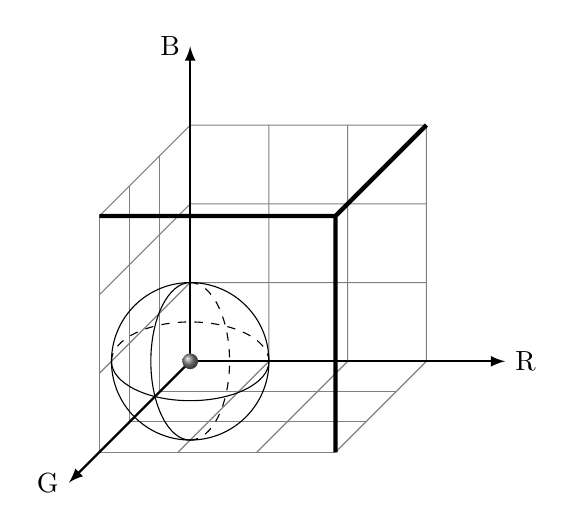
\begin{tikzpicture}
    \def \radi{3}
    \def \x{3}
    \def \y{3}
    \def \z{3}

    \begin{scope}
     \begin{scope}[color=gray, thin]
      \foreach \xi in {0,...,\radi}{ \draw (\xi,\radi,0) -- (\xi,0,0) -- (\xi,0,\radi); }%
      \foreach \yi in {1,...,\radi}{ \draw (0,\yi,\radi) -- (0,\yi,0) -- (\radi,\yi,0); }%
      \foreach \zi in {0,...,\radi}{ \draw (0,\radi,\zi) -- (0,0,\zi) -- (\radi,0,\zi); }%
     \end{scope}

     \draw[-latex, thick, color=black] (0,0,0) -- (4,0,0) node[anchor=west] {R};%
     \draw[-latex, thick, color=black] (0,0,0) -- (0,4,0) node[anchor=east] {B};%
     \draw[-latex, thick, color=black] (0,0,0) -- (0,0,4) node[anchor=east] {G};%

     \draw[color=black, ultra thick]
     (0,\y,\z) -- (\x,\y,\z) -- (\x,\y,0) (\x,\y,\z) -- (\x,0,\z);
    \end{scope}

    \draw (-1,0) arc (180:360:1cm and 0.5cm);
    \draw[dashed] (-1,0) arc (180:0:1cm and 0.5cm);
    \draw (0,1) arc (90:270:0.5cm and 1cm);
    \draw[dashed] (0,1) arc (90:-90:0.5cm and 1cm);
    \draw (0,0) circle (1cm);
    \shade[ball color=gray,opacity=1] (0,0) circle (0.1cm);
   \end{tikzpicture}
   \caption{Color neighborhood represented in a RGB orthogonal three-dimensional color space.}
   \label{figure:rgb_space}
\end{figure}

\newpage

% subsection color_difference_evaluation (end)

\subsection{Color blob detection} % (fold)
\label{sub:tracking_library_for_the_web:color_tracking_algorithm:color_blob_detection}

Once all pixels of the tracked color are collected two steps are still required: (1) Detect outliers; and (3) Find the coordinates that represent the color blob.

\subsubsection{Detecting outliers}
\label{sub:tracking_library_for_the_web:color_tracking_algorithm:color_blob_detection:detecting_outliers}

Outliers pixels are determined if they are not close enough to other pixels with the same characteristics. For each pixel $p=(x,y)$, the mean distance with the other found pixels is calculated as follows:

$$meanDistance=\frac{\sum_{1}^{n}\sqrt{(x_n-x)^2 + (y_n-y)^2}} {n},$$

If the $meanDistance$ is greater than a $blobThreshold=30$ the tested pixel is considered ``too far'' from the color blob and is discarded (outlier). The non-discarded pixels (inliers) are in average closer than $blobThreshold$ from each other, representing the tracked color blob.

% subsubsection detecting_outliers (end)

\subsubsection{Finding color blob coordinates}
\label{sub:tracking_library_for_the_web:color_tracking_algorithm:color_blob_detection:finding_color_blobs_coordinates}

After the color blob is detected, the found pixels are close enough to represent a color blob. To determine the blob central coordinates $C_b=(x_b,y_b)$, the value for each axis is determined based on the average of each pixel axis value $p_n=(x_n,y_n)$, \ie\ the values of $x_b$ and $y_b$ are calculated as follows:

$$x_b=\frac{\sum_{1}^{n}x_n}{n}, y_b=\frac{\sum_{1}^{n}y_n}{n}.$$

% subsubsection finding_color_blobs_coordinates)

\subsubsection{Discussion}
\label{sub:tracking_library_for_the_web:color_tracking_algorithm:color_blob_detection:discussion}

The described color technique results in a fast and robust solution for color blob detection on the web. On Figure \ref{figure:color_tracking} is shown the result running on the browser with and without possible outliers interference in the scene.

\begin{figure}[!htb]
  \centering
  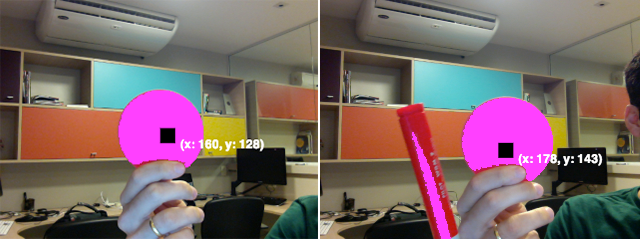
\includegraphics[width=\linewidth]{chapters/tracking_library_for_the_web/color_tracking.png}
  \caption{Example of color tracking technique. The black square represents the central color blob coordinate $C_b$. On the left, the magenta circle is tracked without outliers interference. On the right an outlier object of the same color is introduced in the scene without causing issues to the found circle.}
  \label{figure:color_tracking}
\end{figure}

% subsubsection discussion)

% subsection color_blob_detection (end)

% section color_tracking_algorithm (end)

% chapter tracking_library_for_the_web (end)